\documentclass{report} 
\title{DSP notes 1}
\date{Started April 11th 2024}
\author{Malcolm}
\usepackage{amsmath} %import math
\usepackage{mathtools} %more math
\usepackage{amssymb} %for QED symbol
\usepackage{amsthm} %
\usepackage{bm}%bold math
\usepackage{graphicx} %import imaging
\graphicspath{{./images/}} %set imaging path
\begin{document}
\maketitle

\tableofcontents

\newpage
\section{Convolution algorithm}
We consider two algorithms, the first \textit{input} algorithm considers convolution from the 
viewpont of the input signal---how each input sample contributes to
multiple points. The second considers \textit{output} algorithm does the same but for the output signal---how 
an output sample has received information from multiple input samples.\\
\vspace{1mm}\\
The first perspective demonstrates the conceptual understanding of convolution, while the second the mathematics.
Recall the (continuous) definition of the convolution:
\begin{equation*}
(f*g)(t)=\int^{t^+}_{0^-}f(\tau)g(t-\tau)d\tau\quad\text{for }t>0
\end{equation*}
\noindent\textbf{Input side algorithm}\\
Consider a 9 point input signal $x[n]$ passed through a system with a 4 point impulse response $h[n]$.  
The input $x[n]$ is convolved
with $h[n]$ to produce $y[n]$, the system respose to $x[n]$. The convolution amounts to 
\textit{scaling and shifting the impulse response according to each input sample}, and then \textit{adding
them together}.\\
\vspace{1mm}\\
For example, lets say input sample number 4 is $x[4]=1.4$; this contributes an output component of $1.4h(n-4)$, 
essentially
scale the impulse response by 1.4 and shift it four samples to the right. (The input can be represented
as $1.4\delta[n=4]$, which after passing through the system becomes $1.4h[n-4]$ (linearity)).\\
\vspace{1mm}\\
This is repeated for all the input points, so we have 9 output components for 9 input points. We add these 
components together to get the output.\\
(next page)\newpage
\noindent Consider these figures, squares represent the data points that come from the shifted and
scaled input response, and diamonds for the added zeros:
\begin{center}
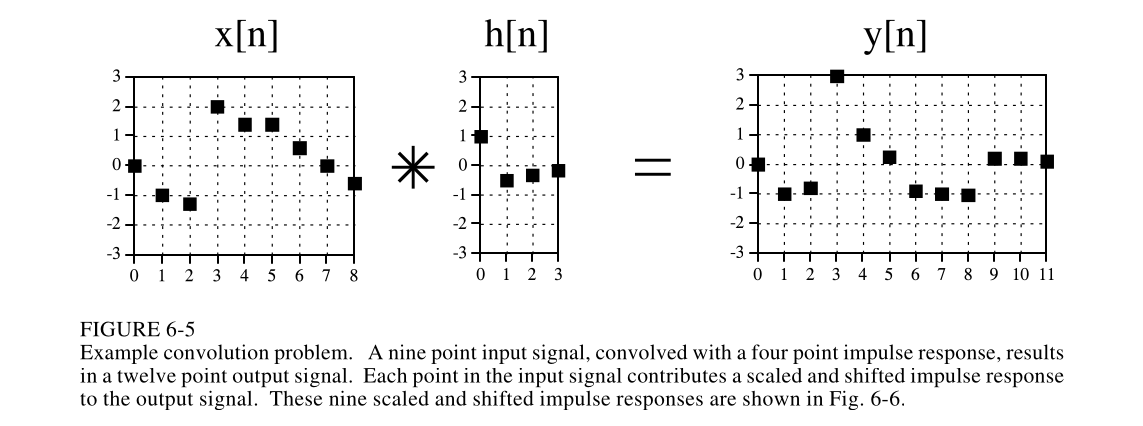
\includegraphics[width=10cm]{a1}\\
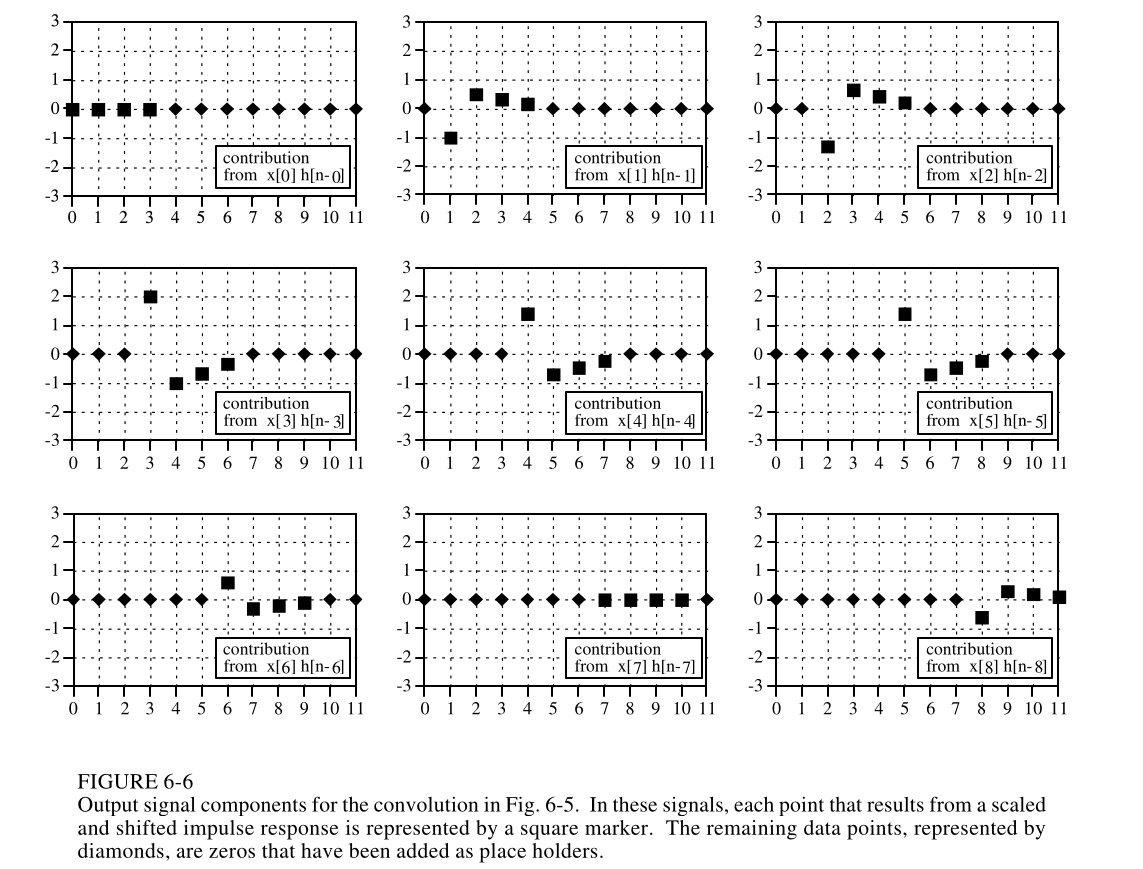
\includegraphics[width=10cm]{a2}\\
\end{center}
The convolution is the resulting sum of the nine scaled and translated impulse responses.\\
\vspace{1mm}\\
To relate this back to the math, intuitively the fourth output point depends on the fourth point of the 
impulse response scaled by the first point of the input, and the third point of the impulse response scaled by 
the second point of the input and so on.









\newpage
\appendix
\chapter{Mathematics (copied from appendices)}

\subsection{Convolution---Definition and properties}
\textbf{Definition}\\
The \textit{convolution} of two functions $f$ and $g$,
denoted by $f*g$, is defined as
\begin{equation*}
(f*g)(t)=\int^{t^+}_{0^-}f(\tau)g(t-\tau)d\tau\quad\text{for }t>0
\end{equation*}
This is a \textit{one-sided} convolution, which is only concerned with functions on the interval $(0^-,\infty)$.\\
\vspace{1mm}\\
\textbf{Properties}\\
\textit{Linearity}; for functions $f_1,f_2,g$ and constants $c_1,c_2$:
\begin{equation*}
(c_1f_1+c_2f_2)*g=c_1(f_1*g)+c_2(f_2*g)
\end{equation*}
This follows from the linearity of integration.\\
\vspace{1mm}\\
\textit{Commutivity}: $f*g=g*f$. This follows from the change of variable $v=t-\tau$; the limits become
\begin{equation*}
\tau=0^-\implies t-\tau=t^+\quad\text{and}\quad\tau=t^+\implies t-\tau=0^-
\end{equation*}
\textit{Associativity}: $f*(g*h)=(f*g)*h$. Showing this amounts to changing the order of integration. 
First consider the discrete case:
\begin{align*}
((f*g)*h)(n)&=\sum^n_{k=0}(f*g)(k)h(n-k)\\
&=\sum^n_{k=0}\left(\sum^k_{i=0}f(l)g(k-l)\right)h(n-k)\\
&=\sum_{0\leq l\leq k\leq n}f(l)g(k-l)h(n-k)\\
&=\sum^n_{l=0}\sum^n_{k=l}f(l)g(k-l)h(n-k)\\
&=\sum^n_{l=0}f(l)\left(\sum^{n-1}_{k=0}g(k)h(n-k-l)\right)\\
&=\sum^n_{l=0}f(l)(g*h)(n-l)\\
&=(f*(g*h))(n)
\end{align*}
(next page)\newpage
\noindent\textbf{Properties cont.}\\
The continuous case is analogously:
\begin{align*}
((f*g)*h)(t)&=\int^t_0(f*g)(s)h(t-s)ds\\
&=\int^t_{s=0}\left(\int^s_{u=0}f(u)g(s-u)du\right)h(t-s)ds\\
&=\iint_{0\leq u\leq s\leq t} f(u)g(s-u)h(t-s)du\,ds\\
&=\int^t_{u=0}f(u)\left(\int^{t-u}_{s=0}g(s)h(t-u-s)ds\right)du\\
&=\int^t_{u=0}f(u)(g*h)(t-u)du\\
&=(f*(g*h))(t)
\end{align*}
\textbf{Delta functions}\\
See that
\begin{equation*}
(\delta*f)(t)=f(t)\quad\text{and}\quad(\delta(t-a)*f)(t)=f(t-a)
\end{equation*}
These can be shown via direct computation. Recall that for $b>0$
\begin{equation*}
\int^b_{0^-}\delta(\tau)f(\tau)d\tau=f(0)
\end{equation*}
So it follows that for $t\geq0$
\begin{align*}
(\delta*f)(t)&=\int^{t^+}_{0^-}\delta(\tau)f(t-\tau)d\tau=
f(t-0)=f(t)\\
(\delta(t-a)*f)(t)&=\int^{t^+}_{0^-}\delta(\tau-a)f(t-\tau)d\tau=f(t-a)
\end{align*}
(for the second statement see that the delta function only has magnitude for $\tau=a$) 
\newpage

\subsection{Green's Formula}
\textbf{Definition}\\
Suppose we have the linear time invariant system with rest initial conditions:
\begin{equation*}
p(D)y=f(t),\quad y(t)=0\text{ for }t<0
\end{equation*}
Suppose that $w(t)$ is the unit impulse response (also called the \textit{weight} function) for the above system. 
That is, $w(t)$ satisfies $p(D)w=\delta(t)$,
with rest initial conditions. \textit{Green's formula} states that for any input $f(t)$ the solution to that
system is given by
\begin{equation*}
y(t)=(f*w)(t)=\int^{t^+}_{0^-}f(\tau)w(t-\tau)d\tau
\end{equation*}
This means we can find the response to \textit{any} input once we know the unit impulse response. It is also
an integral, which can be computed numerically if necessary.\\
\textbf{Intuition}\\
Recall that linear time invariance means 
\begin{equation*}
y(t)\text{ solves }p(D)y=f(t)\implies y(t-a)\text{ solves }p(D)y=f(t-a)
\end{equation*}
(If $y(t)$ is the response to input $f(t)$ then $y(t-a)$ is the response to input $f(t-a)$.) 
First consider partitioning time into intervals of width $\Delta t$; so $t_0=0,t_1=\Delta t,t_2=2\Delta t$, etc.:
\begin{center}
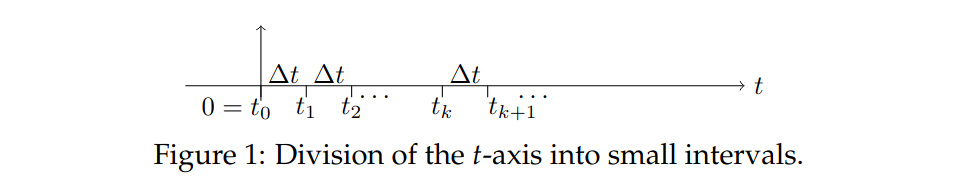
\includegraphics[width=10cm]{56}\\
\end{center}
Next we decompose the input signal $f(t)$ into packets over each interval. The $k$th signal packet, $f_k(t)$
coincides with $f(t)$ between $t_k$ and $t_{k+1}$ and is 0 elsewhere:
\begin{equation*}
f_k(t)=\begin{cases}
f(t)&\text{for }t_k<t<t_{k+1}\\
0&\text{elsewhere}
\end{cases}
\end{equation*}
\begin{center}
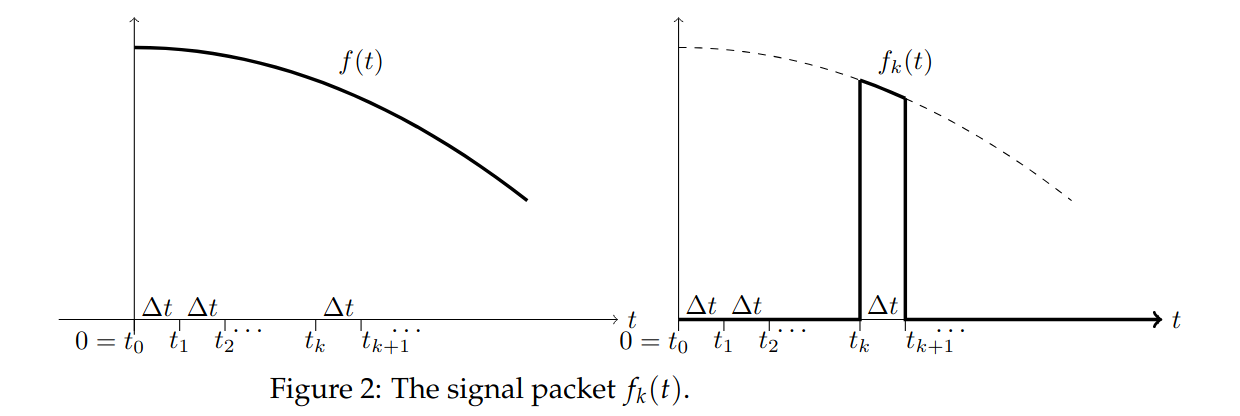
\includegraphics[width=10cm]{57}\\
\end{center}
(next page)\newpage
\noindent\textbf{Intuition cont.}\\
Naturally for $t>0$ we have $f(t)$ as the sum of the packets
\begin{equation*}
f(t)=f_0(t)+f_1(t)+\ldots+f_k(t)+\ldots
\end{equation*}
Given that a single packet $f_k(t)$ is concentrated entirely in the small neighbourhood of $t_k$, they can be
approximated as an impulse with the same size as the area under $f_k(t)$, we also approximate the 
area as a rectangle, (like a riemann sum) so 
\begin{equation*}
f_k(t)\approx(f(t_k)\Delta t)\delta(t-t_k)
\end{equation*}
The weight function $w(t)$ is the response to $\delta(t)$. So by linear time invariance the response to $f_k(t)$ is
\begin{equation*}
y_k(t)\approx(f(t_k)\Delta t)w(t-t_k)
\end{equation*}
Say we want to find the response at a fixed time $T$, we
know $f$ (input) is the sum of $f_k$ so by \textit{superposition}
we have $y$ (output) as the sum of $y_k$. At time $T$:
\begin{align*}
y(T)&=y_0(T)+y_1(T)+\ldots\\
&\approx\left(f(t_0)w(T-t_0)+f(t_1)w(T-t_1)+\ldots\right)\Delta t
\end{align*}
We can ignore all the terms where $t_k>T$ as $T-t_k<0$ so $\delta(T-t_k)=0$ and $w(T-t_k)=0$. So
if $n$ is the last index where $t_k<T$ we have
\begin{equation*}
y(T)\approx\left(f(t_0)w(T-t_0)+f(t_1)w(T-t_1)+\ldots+
f(t_n)w(T-t_n)\right)\Delta t
\end{equation*}
This is a riemann sum; as $\Delta t\to0$ it tends to the integral
\begin{equation*}
y(T)=\int^T_0f(t)w(T-t)dt
\end{equation*}
which is the convolution $(y*w)(T)$---the system response is the convolution of the input with the impulse response.




\end{document}
